\documentclass[11pt]{article}
\usepackage[pdftex]{graphicx}
\usepackage[explicit]{titlesec}
\usepackage[OT1]{fontenc}
\usepackage[most]{tcolorbox}
\usepackage[final]{pdfpages}
\usepackage[colorlinks=true, urlcolor=cyan, hyperfootnotes=false]{hyperref}
\usepackage{fullpage, graphicx, psfrag, url, caption, authblk, amsfonts, amsmath, amssymb, float, fancyhdr, multicol, cmbright, xcolor, amsthm, gensymb, physics, comment}

\fancypagestyle{pages}{
	%Headers
	\fancyhead[L]{Physics 7A, Summer 2024 \\ Section 103}
	%\fancyhead[C]{\thepage}
	\fancyhead[R]{Discussion 8 \\ July 8}
\renewcommand{\headrulewidth}{0pt}
	%Footers
	%\fancyfoot[L]{}
	\fancyfoot[C]{}
	\fancyfoot[R]{\thepage}
\renewcommand{\footrulewidth}{0pt}
}

\newcommand\blfootnote[1]{
    \begingroup
    \renewcommand\thefootnote{}\footnote{#1}
    \addtocounter{footnote}{-1}
    \endgroup
}

\newcommand{\fig}[4]{
    \begin{figure}[H]
        \centering
        \includegraphics[scale={#3}, angle={#4}]{#1}
        \caption{#2}
        \label{exp4fit}
    \end{figure}
}

\newtheoremstyle{gangnamstyle}{}{}{}{}{\sffamily\bfseries}{.}{ }{}
\tcolorboxenvironment{definition}{boxrule=0pt,boxsep=0pt,colback={blue!10},left=8pt,right=8pt,enhanced jigsaw, borderline west={2pt}{0pt}{blue},sharp corners,before skip=10pt,after skip=10pt,breakable}
\tcolorboxenvironment{example}{boxrule=0pt,boxsep=0pt,colback={orange!10},left=8pt,right=8pt,enhanced jigsaw, borderline west={2pt}{0pt}{orange},sharp corners,before skip=10pt,after skip=10pt,breakable}
\tcolorboxenvironment{problem}{boxrule=0pt,boxsep=0pt,colback={cyan!10},left=8pt,right=8pt,enhanced jigsaw, borderline west={2pt}{0pt}{cyan},sharp corners,before skip=10pt,after skip=10pt,breakable}
\theoremstyle{gangnamstyle}{\newtheorem{definition}{Definition}[]}
\theoremstyle{gangnamstyle}{\newtheorem{example}{Example}[]}
\theoremstyle{gangnamstyle}{\newtheorem{problem}{Problem}[]}

\headheight=0pt
\footskip=0pt
\setlength{\oddsidemargin}{0 in}
\setlength{\evensidemargin}{0 in}
\setlength{\topmargin}{-0.5 in}
\setlength{\textwidth}{6.5 in}
\setlength{\textheight}{8.5 in}
\setlength{\headsep}{0.75 in}
\setlength{\parindent}{0 in}
\setlength{\parskip}{0.1 in}

\begin{document}
\normalfont
\pagestyle{pages}

% Begin Document

\begin{center}
\vspace{3in}
{\Large Discussion 8 } \\ [0.05in]
Midterm 1 Review \\ [-0.5in]
\end{center}

\section*{Topics}
\begin{itemize}
\item Kinematics
\item Dynamics
\item Uniform Circular Motion
\end{itemize}
All the problems are taken from past exams, most of which come from Berkeley TBP's website. 

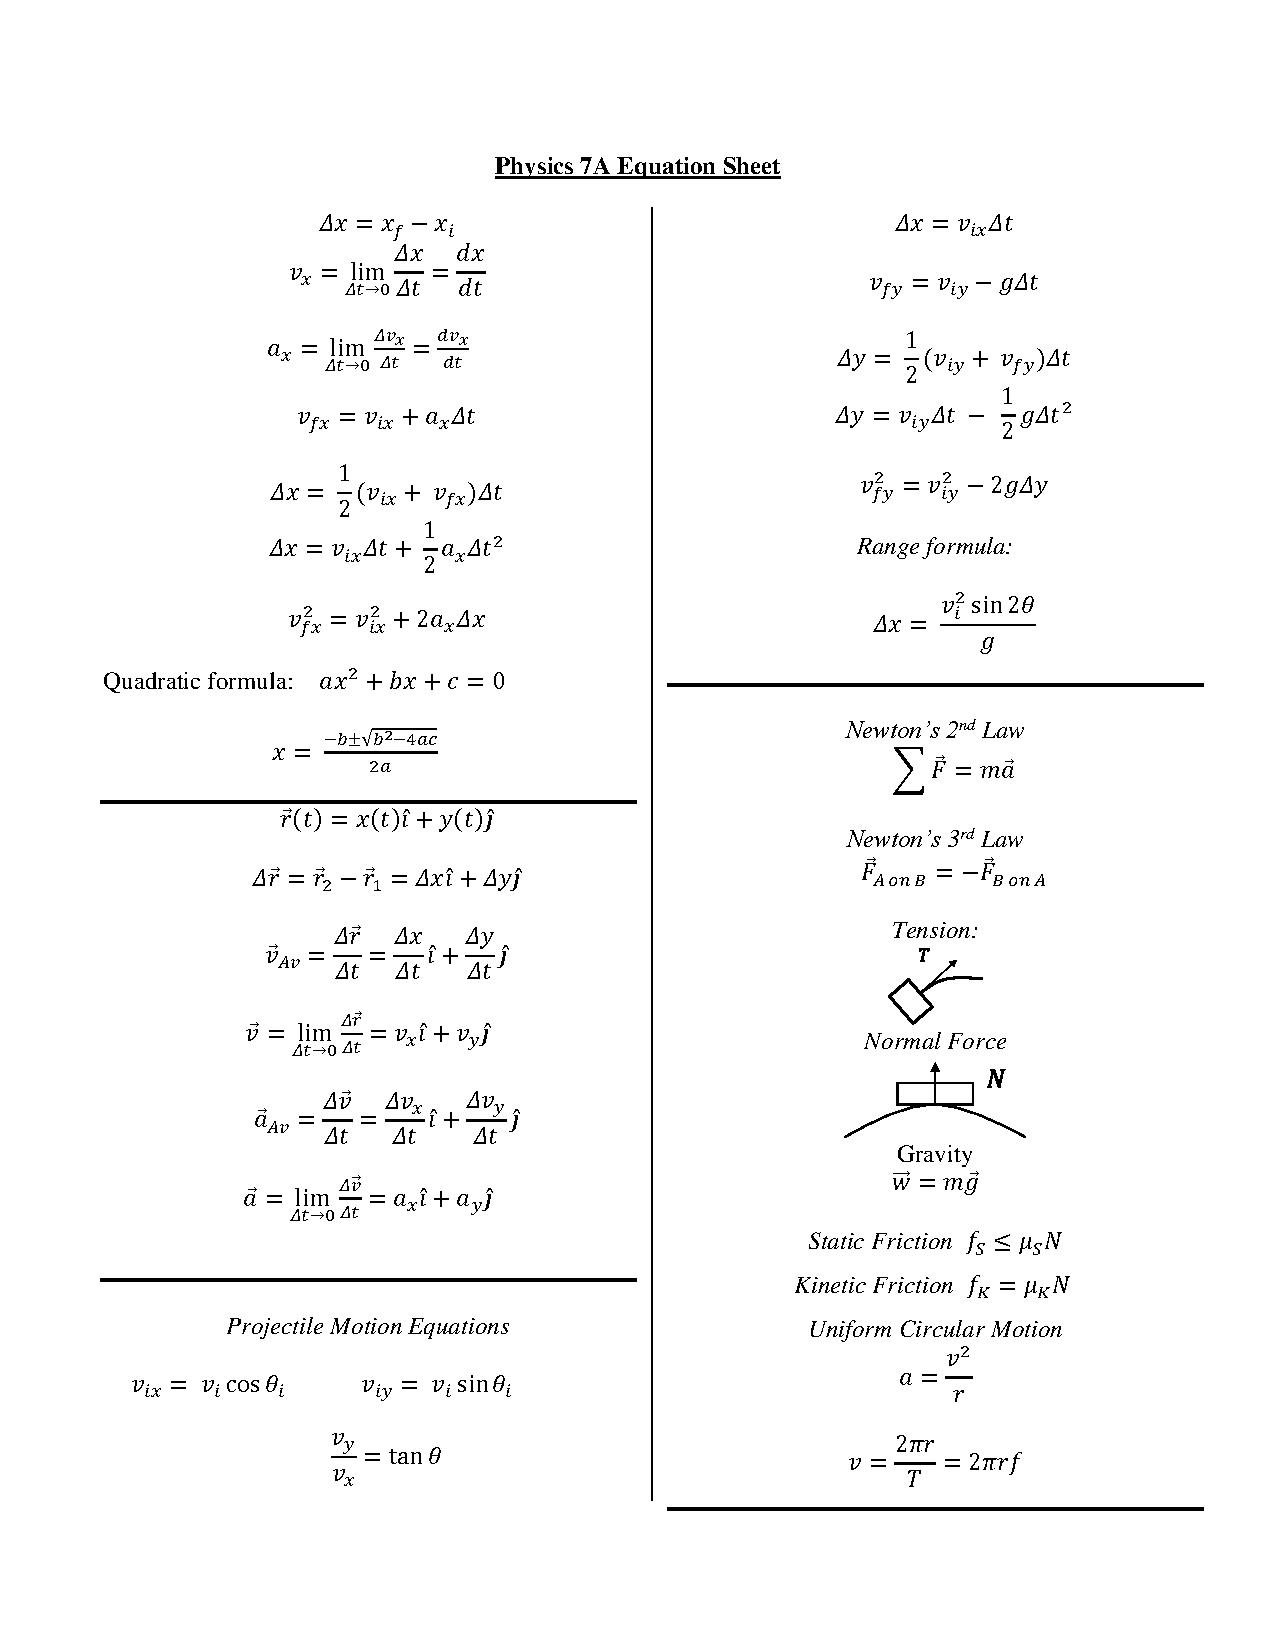
\includepdf[pages=-]{figs/0708/equation.pdf}

\section{Kinematics}

\textbf{1.} \textit{Taken From Fall 2018 (Stahler)} 

A ball is launched at point $O$, which lies a distance $D$ from a vertical wall. The initial speed of the ball is $v_0$, and the initial launch angle is $\theta_0$, as shown. Embedded in the vertical wall is a small pipe, located a height $H$ above the ground. In order for the ball to enter the pipe, its velocity must be in the horizontal direction. Your task will be to find the initial angle $\theta_0$ such that the ball enters the pipe. Proceed in the following steps:

\fig{figs/0708/pipe.png}{Ball and Pipe}{0.4}{0} 

(a) Find an expression for $v_{0y}$, the initial vertical speed, in terms of $g$ and $H$. 

(b) Next find a second expression for $v_{0y}$ in terms of $g$, $D$, and $v_{0x}$, the initial horizontal speed. 

(c) Find $v_{0x}$ in terms of $g$, $D$, and $H$. 

(d) Find $\theta_0$ in terms of $D$ and $H$.

\pagebreak

\begin{center}
(Blank Page)
\end{center}

\pagebreak

\section{Dynamics}

\textbf{1.} \textit{Taken From Fall 2014 (DeWeese)} 

A weight of mass $M$ is suspended by two ideal ropes with tension $T_1$, $T_2$, at angles $\theta_1$, $\theta_2$ from the horizontal. 

\fig{figs/0708/block.jpeg}{Mass and Ropes}{0.125}{0} 

In part (a), do not assume $\theta_1 = \theta_2$. 

(a) If nothing is moving, find $T_1$ in terms of $M$, $\theta_1$, $\theta_2$. 

In parts (b) - (e), let $\theta_{1, 2}$ be equal. Denote $\theta = \theta_1 = \theta_2$. 

(b) If nothing is moving, what is $T_1$ in terms of $T_2$? 

(c) If the system containing both ropes and the mass are accelerating straight up with an acceleration $a$, then what is $T_1$? 

(d) If the system containing both ropes and the mass are accelerating straight to the right with an acceleration of $a$, then what is $T_1$? 

(e) What is the maximum value of $a$ in the scenario of part (d)? 

\pagebreak

\begin{center}
(Blank Page)
\end{center}

\pagebreak

\section{Uniform Circular Motion}

\textbf{3.} \textit{Taken From Fall 2008 (Speliotopoulos)} 

A block slides in a circle within a bowl (see figure). The speed of the block is constant, and all surfaces are frictionless. What must the cross-sectional shape of the bowl be so that the time it takes the block to go around the circle once does not depend on its speed? In other words, how must the height, $y$, of the block depend on the radius, $r$, of the circle its path makes?
\fig{figs/0708/bowl.png}{The Bowl}{0.4}{0} 

\pagebreak

\begin{center}
(Blank Page)
\end{center}

\pagebreak

\begin{comment}
\section{The "Extra Credit" Problem}
\textit{This problem is very challenging and may require a lot of time (perhaps over 1 hour) to solve. Do not attempt it unless you have exhausted the other practice problems.} \textit{If I were the professor, I could most likely put a very hard problem on the exam and call it "extra credit". Sadly, I am merely your teaching assistant, and I can only give you brownie points for solving it.} 

\textbf{4.} \textit{Taken From Spring 2023 (Charman)} 

Workers hope to haul a crate (the “load”) of initial mass $M_1 = M$ up a frictionless hill (of $30\degree$ slope) with the help of a steel cable connecting this load to a counterweight of mass $M_2 = \frac{2}{3}M$ on the other, steeper side of the hill ($60\degree$ slope), also frictionless. The cable is thin, flexible but inextensible, and uniform, of total length $L$, but of non-negligible mass $m = \frac{1}{3}m$. The hill is near sea level, but air resistance may be neglected. 

Let $s$ represent the length of cable on the left side of the hill. Assume that the cable always remains taught and parallel to the hillsides, except where it bends very sharply around the (frictionless) apex of the hill, which effectively acts as an ideal pulley. The hill is tall enough that neither mass can reach the bottom while the masses remain connected by the cable but located on opposite sides of the hill. 

\fig{figs/0708/triangle.png}{Two Masses Connected by a Steel Cable on a Frictionless Hill}{0.75}{0} 

After getting everything connected, suppose that the workers pause a lunch while the masses remain at rest: 

(a) How much of the cable is on the left hand side of the hill? Express this length $s$ as a function of $L$ and any other needed quantities.

(b) What is the magnitude of the tension in the cable, at the very top of the mountain? Express your answer in terms of $M$, $g$, and any other needed quantities.

(c) What is the magnitude of the tension in the cable where it connects to the load? Express your answer in terms of $M$, $g$, and any other needed quantities.

\pagebreak

Alas, while the workers are still enjoying their lunch break, the crate breaks open, suddenly dumping part of its contents, and leaving the crate with mass $M' = \frac{1}{3}M$. After this sudden loss of part of the mass, but before the crate reaches the top of the hill: 

(d) Find the acceleration $a$ of the crate as a function of its position along the hillside. Express your answer as a function of $s$, $M$ , $L$, $g$, and any other needed quantities, in terms of either a magnitude and direction, or horizontal and vertical components.

(e) For a given value of $s$, where along the cable is the tension the greatest (in magnitude)? What is the magnitude of the tension there? Express your answer in terms of $s$, $M$, $L$, $g$, and any other needed quantities.

(f) Find the speed of the crate just as it reaches the top of the hill. 

\pagebreak

\begin{center}
(Blank Page)
\end{center}

\pagebreak
\end{comment}

\end{document}
